 % compile: pdflatex  -shell-escape Erlang_Jevtic_Mrdak_Dimic_Gajic.tex
% !TEX encoding = UTF-8 Unicode

\documentclass[a4paper]{article}

\usepackage{color}
\usepackage{url}
\usepackage[T2A]{fontenc} % enable Cyrillic fonts
\usepackage[utf8]{inputenc} % make weird characters work
\usepackage{graphicx}
\usepackage{amsthm}
\newtheorem{definition}{Definicija}

\usepackage[english,serbian]{babel}

\usepackage[unicode]{hyperref}
\hypersetup{colorlinks,citecolor=green,filecolor=green,linkcolor=blue,urlcolor=blue}

\newtheorem{primer}{Primer}[section]

\usepackage{minted}
\usemintedstyle{colorful}

\usepackage{tikz}
\def\checkmark{\tikz\fill[scale=0.4](0,.35) -- (.25,0) -- (1,.7) -- (.25,.15) -- cycle;}

\usepackage{listings}
\lstset{language=erlang}

\begin{document}

\title{Erlang - funkcionalno rešenje za konkurentni svet\\ \small{Seminarski rad u okviru kursa\\Metodologija stručnog i naučnog rada\\ Matematički fakultet}}

\author{Tijana Jevtić, Jelena Mrdak, David Dimić, Zorana Gajić\\
tijanatijanajevtic@gmail.com, mrdakj@gmail.com,\\daviddimic@hotmail.com, zokaaa\_gajich@bk.ru}
\date{6.~april 2019.}
\maketitle

\abstract{

Nakon čitanja rada, čitalac će imati globalnu sliku o jeziku i detaljniji pogled na neke važne koncepte, 
kao i uvid u korišćenu literaturu koju može konsultovati radi daljeg informisanja o temi.

% Pocetak onaj sam ubacila u uvod, msm da mu je tamo mesto!
%TODO ovu recenicu bih mozda ostavila za kraj abstrakta, samo da se ne kaze detaljniji pogled na neke vazne koncepte vec "i detaljan pogled na osnovnu specificnost jezika"
%TODO 1. Problem i glavne rezultate
% 			 2. Motivacija - zasto je tema interesantna i vazna, kako utice na nas. (poglavlje 3 + mozda reci "pokazacemo vam zasto bas ovaj jezik koriste svetske kompanije" kao neku motivaciju)
%		     3.	 Cilj i svrha rada - da ubedimo citaoce da je Erlang veoma super zgodan jezik za funkcionalno programiranje, da docaramo moc jezika

\setcounter{tocdepth}{1} 
\tableofcontents

\newpage

\section{Uvod}
\label{sec:uvod}
%TODO 1. Zaintrigirati !
%			 2. Navesti siru oblast i sam problem koji je tema rada konkretnije 
% 			 3. Sumirati relevantna postignuca na datu temu, reci sto su bitna i interesantna
% 			 4. Sta je ono sto nije uradjeno u oblasti - ne nasem radu, nego u programskom jeziku
% 		      5. Cilj rada, pristup resenju i glavne rezultate.
% 			 6. Najaviti sta ce biti u radu - poglavlja, poslednji pasus uvoda. 

U ovom radu je prikazan programski jezik Erlang iz različitih uglova.
Kroz niz poglavlja i primera, ispričana je njegova istorija - kad, kako, gde i zašto je nastao, 
po čemu je karakterističan, šta ga to izdvaja od drugih programskih jezika, koji su to 
koncepti koji su svojevrsni Erlangu. 

Akcenat će biti na funkcionalnoj paradigmi i uobičajenim mehanizmima koji funkcionalni jezici implementiraju, kao što su: sakupljači otpadaka, poklapanje obrazaca, načini izračunavanja izraza itd.

%TODO Mozemo pocetak za pogavlja ovako 
Kroz niz poglavlja i primera, ispričana je njegova istorija - kad, kako, gde i zašto je nastao \ref{sec:nastanak}, po čemu je karakterističan i koja mu je osnovna namena \ref{sec:namena} \ref{sec:osobine}. 
% ili ovako
Na samom početku rada u poglavlju \ref{sec:nastanak} ćemo se upoznati sa istorijskim razvojem jezika. Nešto više reči o nameni, mogućnostima i osnovnim osobinama Erlang-a će biti u poglavljima \ref{sec:namena} \ref{sec:osobine}. U narednom poglavlju \ref{sec:konkurentnost} posvetićemo posebnu pažnju konkuretnosti. Onda ćemo videti uticaj Erlang-a u veb programiranju, upoznaćemo se sa veb okruženjima ChicagoBoss, Nitrogen i Zotonic u poglavlju \ref{sec:okruzenja}. Sekcija \ref{sec:instalacija} je posvećena instalaciji i pokretanju Erlang-a, nakon čega sledi sekcija \ref{sec:primeri} sa primerima kodova.

\section{Nastanak i istorijski razvoj}
\label{sec:nastanak}
1981. godine je oformljena nova laboratorija, Erikson CSLab (eng.~{\em The Ericsson CSLab}) u okviru firme Erikson sa
ciljem da predlaže i stvara nove arhitekture, koncepte i strukture za buduće softverske sisteme.
Eksperimentisanje sa dodavanjem konkurentnih procesa u programski jezik Prolog je bio jedan
od projekata Erikson CSLab-a i predstavlja začetak novog programskog jezika.
Taj programski jezik je 1987. godine nazvan Erlang
\footnote{Erlang je jedinica saobraćaja u oblasti telekomunikacija 
i predstavlja kontinuirano korišćenje jednog kanala 
(npr. ako jedna osoba obavi jedan poziv telefonom u trajanju od sat vremena, 
tada se kaže da sistem ima 1 Erlang saobraćaja na tom kanalu).}.    
Sve do 1990., Erlang se mogao posmatrati kao dijalekt Prologa. Od tada, Erlang
ima svoju sintaksu i postoji kao potpuno samostalan programski jezik.
Godine rada su rezultirale u sve bržim, boljim i stabilnijim verzijama jezika, kao
i u nastanku standardne biblioteke OTP (eng.~{\em The Open Telecom Platform}) \cite{phdthesis}.
Od decembra 1998. godine, Erlang i OTP su postali deo slobodnog softvera (eng.~{\em open source software})
i mogu se slobodno preuzeti sa Erlangovog zvaničnog sajta \cite{sajt}.
Danas, veliki broj kompanija koristi Erlang u razvoju
svojih softverskih rešenja. Neke od njih su: Erikson, Motorola, Votsap (eng.~{\em Whatsapp}), 
Jahu (eng.~{\em Yahoo!}), Amazon, Fejsbuk (eng.~{\em Facebook}).


\subsection{Uticaji}
\label{subsec:uticaji}
Erlang je funkcionalan i konkurentan programski jezik.
Na njega, kao na funkcionalan jezik, uticao je Lisp funkcionalnom paradigmom koju je 
prvi predstavio. Na planu konkurentnosti Erlang je svojevrstan primer (detaljnije u poglavlju \ref{sec:osobine}). \\ 

Na početku, Erlang je stvaran kao neki dodatak na Prolog, vremenom prerastao u 
dijalekt Prologa, a kasnije je zbog svoje kompleksnosti i sveobuhvatnosti evoluirao
u potpuno novi programski jezik. Stoga je uticaj Prologa na Erlang bio 
neminovan. Sintaksa Erlanga u velikoj meri podseća na Prologovu 
(npr. promenljive moraju počinjati velikim slovom, 
svaka funkcionalna celina se završava tačkom), oba jezika u velikoj meri koriste poklapanje obrazaca
(eng.~{\em pattern matching}). \\

Sa druge strane, Erlang je uticao na nastanak programskog jezika Eliksir (eng.~{\em Elixir}). Eliksir,
uz izmenjenu Erlangovu sintaksu, dopunjenu Erlangovu standardnu biblioteku, uživa široku popularnost.


\section{Osnovna namena, svrha i mogućnosti}
\label{sec:namena}
Sa početkom od 1981. godine, jedan od zadataka Eriksonove laboratorije za računarstvo je bio pronalaženje načina za bolje programiranje aplikacija
za telekomunikacije \cite{phdthesis}. Takve aplikacije su ogromni programi i od velike važnosti je da rade sve vreme (koliko je to moguće). 
Naravno, poznato je da će tolika količina koda zasigurno imati greške, ali u toj vrsti industrije, greške mogu biti fatalne. Na primer, 
šta se dešava ako je došlo do kvara na nekoj telefonskoj liniji, a telefon nam je hitno potreban (recimo, neko ima srčani udar).
Jednostavno nije moguće zaustaviti takvu aplikaciju, popraviti je i nanovo pustiti u rad.
Kako se izboriti sa greškama u softverskim sistemima kada su one neminovne je osnovna motivacija za razvoj Erlanga \cite{phdthesis}. \\

Tako, jedna od njegovih namena jeste pisanje što sigurnijih programa koje je moguće popraviti bez potrebe za isključivanjem čitavog sistema \cite{book_joe}.
Vrlo brzi konkurentni i distribuirani programi su još jedna od Erlangovih specijalnosti. 
Poseban koncept konkurentnosti koji je implementiran u Erlangu (više u poglavlju \ref{sec:konkurentnost}), kao i funkcionalna paradigma 
omogućavaju lako skaliranje programa i pravljenje velikih konkurentnih i distribuiranih sistema.
Velika zajednica koja se godinama razvijala je doprinela stvaranju velikog broja biblioteka i okruženja za Erlang, te proširila njegov 
inicijalni skup mogućnosti i namena \cite{book_joe}. 


\section{Osnovne osobine}
\label{sec:osobine}
Erlang je zasnovan na funckionalnoj i deklarativnoj paradigmi sa akcentom na konkurentnosti. 
Kao pripadnik funkcionalne paradigme poseduje sakupljač otpadaka u realnom vremenu, tako da se ne mogu pojaviti greške programera pri rukovanju memorijom. 
Takođe, sistem ima ugrađenu kontrolu vremena, 
u smislu da se može odrediti koliko će neki proces čekati na poruku pre nego što se aktivira, 
pa omogućava pisanje aplikacija koje rade u mekom realnom vremenu (eng.~{\em soft real-time systems}) sa odzivom od nekoliko milisekudni. 
U ovom poglavlju videćemo koji su tipovi podžani u Erlangu da bi se njegove osibine i namene opisane u poglavlju \ref{sec:namena} ostvarile, 
kao i neka osnovna svojstva i koncepte.



\subsection{Tipovi i promenjive}
Erlang je dinamički jako tipiziran jezik. 
Na raspolaganju nam je 8 primitivnih tipova. 
Osim uobičajnih celobrojnih, realnih vrednosti i referenci, Erlang uvodi i neke specifične tipove kao što su:
\begin{list}{•}{}
\item Atomi koji se pišu malim slovima i predstavljaju konstante i enumerisane tipove. Samo ime je njihova vrednost. Pandan su makroima i enumerisanim tipovima u C-u.
\item Binarne vrednosti omogućavaju lako i čitljivo prelamanje broja na segmente u binarni zapis na zadatoj širini. U oznaci <<vrednost:širina>>
\item Identifikatori procesa predstavljaju reference na procese. Kreiraju se funkcijom spawn
\item Portovi služe za komunikaciju sa spoljašnjim svetom. Ako su u skladu sa protokolom portova preko njih se mogu slati i primati poruke
\end{list}
 
Tu su i dve osnovne strukture koje mogu da sadrže bilo koje tipove: torke $\{elem_1, eleme_2, ... elemt_n\}$ za fiksirani broj elemenata u njima, 
i liste $[elem_1, elem_2, ...]$ za čuvanje promenjivog broja elemenata. 
Osnovni operator konstrukcije liste je $[Glava | Rep]$. 
U okviru listi se prikazuju i niske, za koje ne postoji ugrađeni poseban tip, 
već su one liste vrednost koje odgovaraju vrednostima karaktera. Ako svi elementi liste mogu da se prikažu kao karakteri onda će lista biti ispisana kao niska, što ilustruje naredni primer.
\begin{minted}{erlang}
1> [16#5A, 97+3, 2*50+14, 97, 8#166, 2#1101111].
"Zdravo"
2> [65,97,2].
[65,97,2]
\end{minted}
U drugom primeru 2 se ne može prikazati kao karakter pa lista nije prikazana kao niska. 
Ovde vidimo i neka elementarna izračunavanja i kako sa \# možemo elegantno koristiti bilo koju brojevnu osnovu. 
Da bismo sačuvali izračunavanja potrebne su nam promenjive.\\

Promenjive mogu biti vezane (eng.~{\em bound}), one kojima je ''dodeljena'' neka vrednost, i slobodne. 
Vezivanje se vrši najviše jednom i vrednost vezanih promenjihiv više se ne može menjati (eng.~{\em single assignment variables}) 
osim ako se u interpreteru ne pozove funkicija f() koja sve promenjive načini slobodnim. 
Ovo je u skladu sa idejom funkcionalnih jezika da nema sporednih efekata 
što za posledicu ima jednostavno izvođenje konkurentnosti, 
iako Erlang nije čisto funkcionalan jezik.
Zapravo, operator = ne predstavlja nikakvu dodelu već poklapanje obrazaca.


\subsection{Poklapanje obrazaca}
Većinu funkcija u Erlangu, kao i svako vezivanje promenjivih pišemo putem poklapanja obrazaca. 
Da bismo objasnili ovaj ključni koncept potrebno je prvo da definišemo pojmove terma, obrasca i čuvara.

\theoremstyle{definition}
\begin{definition}{Osnonvni term (eng.~{\em ground term})}
se definiše kao primitivni tip, uređeni par ili lista osnovnog terma.
\end{definition}

\begin{definition}{Obrazac ili šablon (eng.~{\em pattern})}
može biti primitivni tip, promenjiva, uređeni par ili lista šablona.
Ako su u obrascu sve promenjive različite onda se on naziva primitivnim.
\end{definition}

Poklapanje obrazaca (eng.~{\em pattern matching}) je postupak poređenja terma sa obrascem. 
Neformalno\footnote{Formalna definicija u dodatku}, ako obrazac i term imaju isti oblik, poklapanje uspeva, pri čemu će svaka promenjiva biti vezana sa podatkom na njemu odgovarajućoj poziciji. 
Ovaj proces poznat je kao {\em unifikacija}. 
Pri unifikaciji na raspolaganju je i posebna anonimna promenjiva koja se označava sa \_ , a koju koristimo kada nas neka vrednost ne zanima i ne želimo ni jednu promenjivu da vežemo za tu vrednost. U sledećem primeru prve tri linije pokazuju uspešnu unifikaciju, dok je u poslednjoj pokušana unifikacija X sa 51, što nije uspelo kako je X već vezano za \{137, 42\}.

\begin{minted}{erlang}
1> Z = 2.
2> {X, macka} = {{137, 42}, macka}.
3> [Glava|_] = [1,2,3,4,5,6].
4> {X, Y} = {51, kuce}.
\end{minted}

\begin{definition}{Čuvari (eng.~{\em guards})}
su izrazi koji sadrže samo predikate oblika A op B odvojeni zarezom pri čemu su op validni binarni operatori poređenja\footnote{Operatori poređenja su: <, =<, >, =>, ==, /=, =:=, =/=}. Izraz sa čuvarima može da se evaluira samo u true ili false.
\end{definition}
Čuvari sa ključnom rečju {\em when} predstavljaju dodatno proširenje mogućnosti poklapanja obrazaca, za izvođenje jednostavnih testova i poređenja u šablonu, kao u primeru funkcije za maksimum dve vrednosti:
\begin{minted}{erlang}
max(X, Y) when X > Y -> X;
max(X, Y) -> Y.
\end{minted}
Sama funkcija je definisana preko pokpalanja obrazaca sa korišćenjem čuvara. U sledećem delu formalizovaćemo šta je funkcija u Erlangu i kako se definiše.


\subsection{Funkcije}
Svaka funkcija može imati više slučajeva odvojenih sa ';' 
do kojih će doći poklapanjem obrazaca ili preko argumenata ili preko čuvara u {\em when} delu koji je opcioni. 
Telo funkcije od niza izraza razdvojenih ','.
Tačkom se završava definicija i odvaja od ostalih funkcija. 
Njihovi primeri i korišćenja biće detaljnije opisani u delu \ref{sec:primeri}.
\begin{minted}{erlang}
ime_funckije(a11, a12, ... a1N) [when g11, g12, ... g1N] -> 
	telo1;
...
ime_funckije(aM1, aM2, ... aMN) [when gM1, gM2, ... gMN] -> 
	teloM.
\end{minted}

Kao u svakom funkcionalnom jeziku funkcije su građni prvog reda, 
tako da ih možemo prosleđivati kao argumente, vraćati kao povratnu vrednost itd. Na raspolaganju su nam i anonimne lamda funkcije koje imaju sledeći oblik:
\begin{minted}{erlang}
fun(a1, a2, ... aN) -> telo end.
\end{minted}

Česte su rekurzivne definicije funkcija, 
ali moramo imati na umu da su najefikasnije repne rekurzivne za koje nije potreban stek. 
Mnoge funkcije u Erlangu dizajnirane su da se vrte u beskonačnim petljama, 
posebno u klijent-server modelu u ulozi servera opisanog u narednom poglavlju \ref{sec:konkurentnost}.


\section{Konkurentnost kao glavna specifičnost}
\label{sec:konkurentnost}
Jedna od osnovnih osobina Erlanga i specifičnost po kojom se izdvaja od drugih jezika je konkurentnost i koncept na kom je zasnovana.
Posmatrajući svet oko
sebe, uviđamo da je on u suštini konkurentan - u istom trenutku se dešava veliki broj procesa \cite{phdthesis}. 
U tom istom trenutku, mi smo sposobni da takav svet pojmimo i odreagujemo na sve što se u njemu dešava. Dakle, mi prirodno razumemo konkurentnost.
Tako se i prirodno nameće potreba za programskim jezikom koji bi omogućavao jednostavno modelovanje sveta kakav on stvarno jeste.

\subsection{Koncept}
Koncept konkurentnosti implementiran u Erlangu se zove konkurentnost slanjem poruka (eng.~{\em message passing concurrency}), šematski prikazan na slici \ref{fig:concurrency}. Ovo podrazumeva postojanje velikog broja procesa koji nikad ne dele memoriju, već komuniciraju isključivo asinhronim slanjem poruka \cite{book_joe}.
Sva izračunavanja se obavljaju u okviru procesa i trebalo bi da sistem bude dizajniran tako da jedan proces radi jedan mali posao.
Važno je napomenuti da procesi u Erlangu nisu procesi operativnog sistema, već Erlanga.
To je moguće zbog toga što se njegovi programi izvršavaju na BEAM virtuelnoj mašini.
Procesi se prave i uništavaju jako brzo, zauzimaju samo onoliko memorije koliko je neophodno (u većini slučajeva vrlo malo)
i ponašaju se isto na svim operativnim sistemima \cite{book_joe}.

\begin{figure}[h!]
\begin{center}
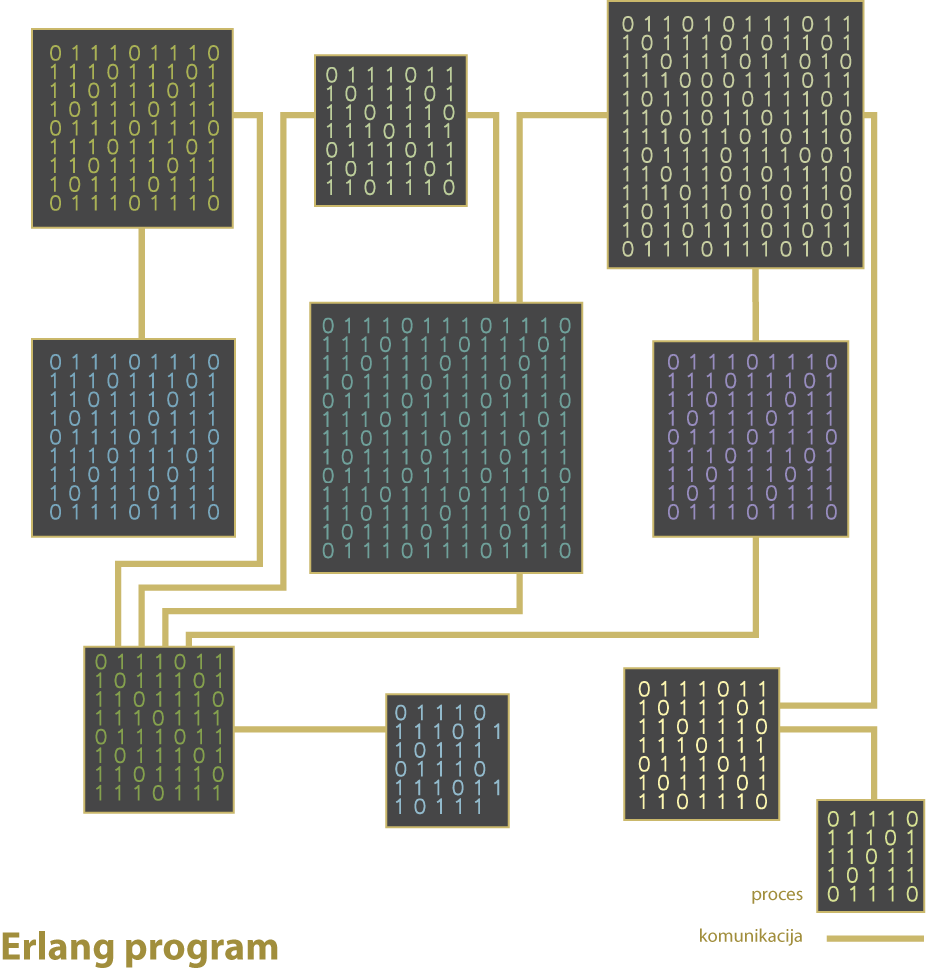
\includegraphics[scale=0.5]{concurrency.png}
\end{center}
\caption{Konkurentnost u Erlangu}
\label{fig:concurrency}
\end{figure} 

Poređenja radi, koncept konkurentnosti korišćen od strane većine programskih jezika je takozvani 
koncept konkurentnosti deljenih stanja (eng.~{\em shared state concurrency}) gde procesi 
menjaju memoriju (nasuprot tome, u Erlangu vrednost promenljivoj može biti dodeljena samo jednom) \cite{book_joe}. 
U slučaju da više procesa žele da menjaju istu memoriju, tzv. kritična sekcija, potrebno je 
nekako zaštiti taj deo memorije (muteksi, katanci i dr.). U slučaju da do greške dođe baš u kritičnoj sekciji,
ostali procesi ne znaju kako da se nose sa datom situacijom i u najboljem slučaju sistem prekida sa radom.

\subsection{Slanje i primanje poruka}
%Slanje
Erlang omogućava jednostavano kreiranje novog procesa pozivom funkcije {\em spawn} koja vraća pid (eng.~{\em process identifier}) na osnovu kojeg svaki proces može da razlikuje ostale procese.
\begin{minted}{erlang}
Pid = spawn([Module], FunctionName, [ArgumentList]) 
\end{minted}

Jedini način za ostvarivanje komunikacije između dva procesa je putem slanja poruka korišćenjem operatora '!'. U {\mintinline{erlang}{Pid ! Message}} procesu sa identifikatorom {\em Pid} šalje se poruka sadržana u promenljivoj {\em Message}, 
pri čemu poruka može biti bilo koji validni term. 
Operator slanja evoluira svoje argumente – prvo levi argument da bi se dobio pid procesa koji prima poruku, 
a potom desni da bi se dobila poruka koja se šalje. 
Povratna vrednost je baš ta poruka.
Slanje poruka je asinhrono, pošiljalac neće čekati da poslata poruka stigne na odredište niti da bude primljena.\\

%Primanje
Za primanje poruka koristi se operator {\em receive}. 
Svaki proces ima svoje sanduče gde se nalaze poruke u redosledu pristizanja. 
Poruke se porede poklapanjem obrazaca. 
Kada poklapanje uspe poruka se vadi iz sandučeta i izvršava se navedena akcija. 
{\em Receive} vraća vrednost poslednjg izraza iz izvršene akcije.
Ako poslata poruka nikad ne stigne na odredište, što se može desiti npr. kao posledica pada procesa koji je poslao poruku, izbegavamo beskonačno čekanje tako što se uvodi maksimalno vreme čekanja (eng.~{\em timeout}).
\begin{minted}{erlang}
receive
    Pattern1 [when Guard1] ->
        Expressions1;
    Pattern2 [when Guard2] ->
        Expressions2;
	... 
	[after Time -> 
		Expressions]
end
\end{minted}

Ukoliko želimo da primimo bilo koju poruku to može da se uradi korišćenjem {\em AnyMessage}. 
Ali, češće želimo da primamo samo one poruke koje su namenjene nama. 
Da bismo to ostvarili moramo poslati svoj pid 
(ako šaljemo pismo moramo napisati svoju adresu da bismo dobili odgovor) 
što se postiže sa funkcijom self().
\begin{minted}{erlang}
Pid ! {self(), Message}
\end{minted}

\subsection{Klijent-server model}
Kada šaljemo poruku procesu moramo znati njegov pid. 
Ovo često nije praktično zbog mogućeg velikog broja procesa, niti poželjno iz bezbedonosnih razloga 
(neki procesi bi trebalo da sakriju svoj identitet). 
Da bi bilo omogućeno slanje poruka bez poznavanja identifikatora uvodi se pojam {\em registrovanja procesa}, tj. davanje imena koje mora biti atom. 
Funkcijom {\mintinline{erlang}{register(name, Pid)}} atom {\em name} se vezuje za {\em Pid} i na dalje ga možemo indentifikovati preko dodeljenog atoma.\\

Glavni razlog registrovanja procesa je da se omogući {\em klijent-server model} koji je ključni za komunikaciju između procesa u Erlangu.
U ovom modelu obe strane mogu biti procesi na istoj ili različitim mašinama. 
Klijent uvek započinje neko izračunavanje obraćajući se serveru, 
koji obrađuje zahtev i vraća odgovor klijentu. Jedan jednostavan primer ovog modela biće objašnjen u delu \ref{sec:primeri}.


\section{Okruženja i njihove karakteristike}
\label{sec:okruzenja}
Erlang je poznat za podržavanje skalabilnih sistema otpornih na greške (eng.~{\em scalable fault-tolerant systems}), ali takođe nudi mnoštvo mogućnosti koje ga čine dobrim jezikom za veb programiranje. Na primer, mogućnost reagovanja na više korisničkih zahteva istovremeno, ne razmišljajući o problemima konkurentnosti.
U tabeli \ref{tab:tabela_okruzenja} je prikazano poređenje 3 glavna veb okruženja: {\em ChicagoBoss}, {\em Nitrogen} i {\em Zotonic} po nekim interesantnim osobinama.

\begin{table}[h!]
\begin{center}
\caption{Poređenje Erlang veb okruženja}
\begin{tabular}{|c|c c c|}\hline
 &ChicagoBoss &Nitrogen &Zotonic \\ \hline
Razvoj zasnovan na događajima &\checkmark  &\checkmark & \checkmark  \\ 
Okruženje za testove &\checkmark  &\checkmark & \checkmark  \\ 
Generisanje koda &\checkmark & - & - \\ 
Django šabloni &\checkmark & - &\checkmark  \\
Integrisani mejl server &\checkmark & - &\checkmark  \\ 
UTF-8 u Erlang kodu &\checkmark & - &\checkmark  \\ 
Višejezični podaci & - & - &\checkmark  \\ 
Generisanje {\em JavaScript} koda & - &\checkmark & \checkmark  \\ 
Generisanje {\em JSON} formata &\checkmark  &\checkmark & \checkmark  \\ 
Integrisani WebSocket &\checkmark  &\checkmark & \checkmark  \\ \hline
 \end{tabular}
\label{tab:tabela_okruzenja}
\end{center}
\end{table} 

Okruženje {\em ChicagoBoss} sadrži sloj apstrakcije baze podataka (eng.~{\em database abstraction layer}) pod nazivom {\em BossDB} \cite{ChicagoBossDocumentation} koji je zaslužan za postavljanje upita nad bazom podataka i njeno ažuriranje. 
Podržani su {\em MySQL, Mnesia, Tokyo Tyrant i PostgreSQL}. 
Za razliku od {\em ChicagoBoss-a}, {\em Nitrogen} okruženje ne podržava model podataka uopšte, dok {\em Zotonic} \cite{ZotonicDocumentation} podržava isključivo {\em PostgreSQL}.\\

Takođe, interesantno je primetiti da neka okruženja imaju integrisani mejl server koji nudi funkcije za primanje i slanje e-pošte i ostale mogućnosti, 
čime olakšava rad korisnicima. 
Na primer, slanje e-pošte u okruženju {\em ChicahoBoss} izgleda ovako:

\begin{minted}{erlang}
boss_mail:send(FromAddress, ToAddress, Subject, Body)
\end{minted} 

U tabeli \ref{tab:tabela_okruzenja} vidimo da sva tri okruženja podržavaju i okruženje za testove, gde su testovi struktuirani kao stabla nastavaka %TODO PREVOD??
 (eng.~{\em trees of continuations}) \cite{EvanMillerTesting}. 
Postoje gotove funkcije koje olakšavaju testiranje nekih opšte poznatih akcija kao što je provera da li je e-pošta ispravno primljena/poslata, da li je stranica na vebu modifikovana itd. \\

{\em Django} šabloni (eng.~{\em Django templates}) \cite{DjangoTempDoc} služe za jednostavnije i brže generisanje dinamičkih HTML stranica pomoću gotovih šablona.
 {\em Nitrogen} ima svoje {\em Nitrogen HTML} šablone ali je u procesu prelazak na {\em Django} šablone.\\
 
Svaki od opisanih okruženja ima svoje prednosti i mane, te zato nije jednostavno presuditi koji od ovih okruženja treba koristiti zasigurno, a koji ne treba. U zavisnosti od onoga šta je prioritet bira se odgovarajuće okruženje. U dodatku \ref{sec:dodatak_primeri_okruzenja} možete pogledati primere u nekim od spomenutih okruženja.

\section{Instalacija i pokretanje}
\label{sec:instalacija}
Postoji više načina da se instalira Erlang sa neophodnim paketima.
Ovde će biti predstavljena instalacija korišćenjem prekompajliranih binarnih fajlova 
za neke operativne sisteme zasnovane na Linuksovom kernelu i pokretanje na jednom od njih, kao i instalacija za Windows.


\subsection{Linux}
\label{subsec:instalacijaLinux}
Na operativnim sistemima zasnovanim na {\em Ubuntu}, Erlang se može instalirati sa:
{\em sudo apt-get install erlang}. 
Nakon uspešne instalacije, Erlang kod je moguće kompajlovati
ili interpretirati i pokretati u interpretatoru.
Interpretator se pokreće kucanjem komande {\em erl} u terminalu, a iz istog
se izlazi sa {\em Ctrl+G} iza kog sledi {\em q} \cite{book_joe}.
Erlang interpretator ima u sebi ugrađen editor teksta koji je baziran na {\em emacs-u} \cite{book_fred}.
K\^od iz datoteke se kompajluje komandom {\em erlc} i navođenjem imena fajla sa ekstenzijom {\em erl}.
Nakon toga se dobija izvršna datoteka sa ekstenzijom {\em beam} koja se može
pokrenuti uz navođenje adekvatnih flegova. 


\subsection{Windows}
\label{subsec:instalacijaWindows}
Na operativnom sistemu {\em Windows}, Erlang se može instalirati preuzimanjem binarne datoteke sa oficijalnog sajta \cite{sajt} programskog jezika. Posle duplog klika na {\em .exe} fajl samo je potrebno ispratiti uputstva. Pokretanje interpretatora se vrši na isti način kao i na Linuks sistemima.


\section{Primeri kodova sa objašnjenjima}
\label{sec:primeri}
Počećemo od jednostavnog primera ''Hello World'' i videti osnovnu sintaksu jezika. 
Jednolinijski komentari počinju znakom \%. 
Prvo navodimo naziv našeg modula u kome se nalaze funkcije koje pišemo, 
a da bi one mogle da se koriste izvan modula potrebno je da ih navedemo u export naredbi. /0 označava da funkcija \textit{start} prima 0 argumenata.
Da bismo željeni tekst prikazali u konzoli, koristimo \textbf{io} modul koji sadrži potrebne IO funkcije u Erlangu.
\begin{minted}{erlang}
% hello world program
-module(helloworld). 
-export([start/0]). 

start() -> 
   io:fwrite("Hello, world!\n").

> Hello, world!
\end{minted}

Kao i većina funkcionalnih jezika, i Erlang podržava shvatanje listi (eng. list comprehensions), što ilustrujemo narednim primerima.
\begin{minted}{erlang}
> [X || X <- [1,2,a,3,4,b,5,6], X > 3].
[a,4,b,5,6]
\end{minted}
Notacija {\mintinline{erlang}{X <- [1, 2, a, ...]}} je generator, dok je izraz {\mintinline{erlang}{X>3}} filter.\\

Možemo primeniti više filtera.
\begin{minted}{erlang}
> [X || X <- [1,2,a,3,4,b,5,6], integer(X), X > 3].
[4,5,6]
\end{minted}

Takođe, moguće je kombinovati i generatore. Na primer, Dekartov proizvod dve liste možemo napisati kao
\begin{minted}{erlang}
> [{X, Y} || X <- [1,2,3], Y <- [a,b]].
[{1,a},{1,b},{2,a},{2,b},{3,a},{3,b}]
\end{minted}

Algoritam QuickSort u Erlangu se može implementirati na sledeći način:
\begin{minted}{erlang}
sort([Pivot|T]) ->
    sort([ X || X <- T, X < Pivot]) ++
    [Pivot] ++
    sort([ X || X <- T, X >= Pivot]);
sort([]) -> [].
\end{minted}
Izraz {\mintinline{erlang}{[X || X <- T, X < Pivot]}} e lista svih elemenata iz T koji su manji od pivota. Slično, {\mintinline{erlang}{[X || X <- T, X >= Pivot]}} je lista svih elemenata iz T koji su veći ili jednaki od pivota.\\

Neizostavna funkcija svih funkcionalnih programskih jezika jeste map.
map(F, List) je funkcija koja prima funkciju F i listu L i vraća novu listu dobijenu primernom funkcije F na svaki element liste L.
\begin{minted}{erlang}
map(F, [H|T]) -> [F(H)|map(F, T)];
map(F, [])    -> [].

double(L)  -> map(fun(X) -> 2*X end, L).

> double([1,2,3,4]).
[2,4,6,8]
\end{minted}


%primer konkurentnost
Naredni primer pokazuje kako komuniciraju procesi u klijent-server modelu opisanog u delu \ref{sec:konkurentnost}.
Klijent šalje zahtev serveru za računanje hipotenuze ili površine pravouglog trougla,
a server vrši izračunavanje u funkciji {\em loop} i vraća odgovoru klijentu. 
Kada modul {\em trougao} bude implementiran, izvršavanje će izgledati ovako: U liniji 1 kreiramo novi serverski proces i dobijemo njegov pid, 
potom ga registrujemo i pozovemo funkciju {\em klijent} koja enkapsulira slanje zahteva i primanje odgovora.
\begin{minted}{erlang}
1> Pid = spawn(fun trougao:loop/0).
2> register(server, Pid).
3> trougao:klijent(server, {hipotenuza,3,4}).
5.0
\end{minted}

U klijentskoj funkciji pošaljilac mora da uključi svoju adresu sa {\em self()} i pošalje zahtev na serverski proces.
Potom čeka odgovor koji je namenjen njemu, odnosno prihvata odgovor kada se poklopi obrazac torke \{Pid, Response\}. Tačnije, {\em Pid} je vezana, a {\em Response} slobodan promenjiva koja će biti vezana kada stigne odgovor.
\begin{minted}{erlang}
klijent(Pid, Request) ->
    Pid ! {self(), Request},
    receive
	{Pid, Response} ->
	    Response
    end.
\end{minted}

Sa klijetske strane takođe se vrši poklapanje obrazaca sa atomom koji je poslat u zahtevu (šta klijent želi da računa), 
izračunavanje i slanje odgovora na adresu klijenta.
Kompletan kod dostupan je u datoteci \href{https://raw.githubusercontent.com/mrdakj/msnr/master/trougao.erl}{trougao.erl}
\begin{minted}{erlang}
loop() ->
    receive
	{From, {hipotenuza, A, B}} -> 
	    From ! {self(), sqrt(A*A + B*B)}, loop();
	{From, {povrsina, A, B}} -> 
	    From !  {self(), A * B / 2}, loop();
	{From, Other} ->
	    From ! {self(), {error, Other}}, loop()
    end.
\end{minted}

\section{Zaključak}
\label{sec:zakljucak}
U ovom radu sažete su i objašnjene najvažnije osobine i paradigme Erlanga. 
Od elementarnih primera i upoznavanja sa sintaksom do njegove pune izražajnosti
kada je u pitanju konkurentnost. 
Elegantan i jednostavan rad sa komunikacijom procesa u potpunosti su opravdali ideju i namenu za koju je jezik nastao.
Kroz izložene koncepte ovaj rad pruža odličan uvod za upoznavanje sa Erlangom i podstek čitaocu na dalje i dublje istraživanje.
%TODO 		 1. Ukratko opisati glavne doprinose rada
%			 2. Sta je to po cemu treba pamtiti rad - konkuretnost, brzina?, sigurnost? jezika
%			 3. Sumirati nalaze, navesti osnovne zakljucke
%			 4. Pravci buduceg razvoja, nove upotrebe, nove mogucnosti - mozda spomenuti primenu u distribuiranim okruzenjima

\addcontentsline{toc}{section}{Literatura}
\appendix
\bibliography{seminarski} 
\bibliographystyle{plain}

\newpage
\appendix
\section{Dodatak}
\subsection{Primeri koda u veb okruženjima}
\label{sec:dodatak_primeri_okruzenja}

U poglavlju \ref{sec:okruzenja} smo se upoznali sa glavnim predstavnicima Erlang veb okruženja i videli njihove osnovne karakteristike. Prikazaćemo nekoliko primera u veb okruženjima. \\ 

Prvo ćemo pokazati jedan napredniji primer od "Hello World" u {\em ChicagoBoss} okruženju. Erlang fajl bi izgledao ovako:
\begin{minted}{erlang}
-module(appname_my_controller, [Req]).
-compile(export_all).
hello('GET', [Name]) ->
	{ok, [{name, Name}]}.
\end{minted}

Dok je u HTML fajlu neophodno napisati:
\begin{minted}{html}
Hello, {{ name }}.
\end{minted} 

Primer u okruženju {\em Nitrogen} sa ispisom poruke kao reagovanje na klik:
\begin{minted}{erlang}
-module(module_name).
-compile(export_all).
-include_lib("nitrogen_core/include/wf.hrl").

main() -> #template{file=template_name}.
title() -> "My Hello World".

body() ->
    #panel{body=[
        "Click on button below!!"
        #br{},
        #button{
            id=button_id_name,
            postback=click,
            text="Click Me"
        }
    ]}.

event(click) ->
    NewBody = #panel{
        id=id_name_of_the_replacement,
        text="You clicked!!"
    },
    wf:replace(button_id_name, NewBody).
\end{minted}


\end{document}
